\chapter{Multimedia Application}
The availability of multimedia hardware and software components has driven the enhancement of existing applications towards being more user-friendly. It has also initiated the continuous development of new multimedia applications.

\section{Video-On-Demand}
Video-On demand (VOD) services represent a class of applications where video information is accessed from one or more video servers.

VOD systems include many more components that are necessary for the provision of a complete service, such as video server(s), administration and maintenance systems, networking services, backbone networks for linking geographically distributed video servers and set-top units for receiving, demodulating, decoding and converting video for television playback.

Elements of a VOD system are shown in Figure \ref{fig:vod}.

The best known application of VOD is the \textit{video library} which uses \textit{Interactive VOD}. Interactive VOD allows a user to gain access to a movie via point-to-point
connection. This connection allows the user individual and instantaneous control of storage medium in terms of \textit{start}, \textit{fast-forward}, \textit{pause} and fast \textit{rewind}.

There are two basic types of interactive VOD service:
\begin{itemize}
	\item \textit{Interactive VOD with instantaneous access}
	
	User can instantly retrieve and individually control program information from a library instantly, with instant control response.
	
	\item \textit{Interactive VOD with delayed access}
	
	User retrieve and individually control program information from a library, but there is a waiting time depending on the available bandwidth resources in the network.
\end{itemize}
%%%%%%%%%%%%%%%%%%%%%%%%%%%%%%%%%%%%%%%%%
%										%
%				FIGURE				   	%
%										%
%%%%%%%%%%%%%%%%%%%%%%%%%%%%%%%%%%%%%%%%%
\begin{figure}[pht!]
	\centering
	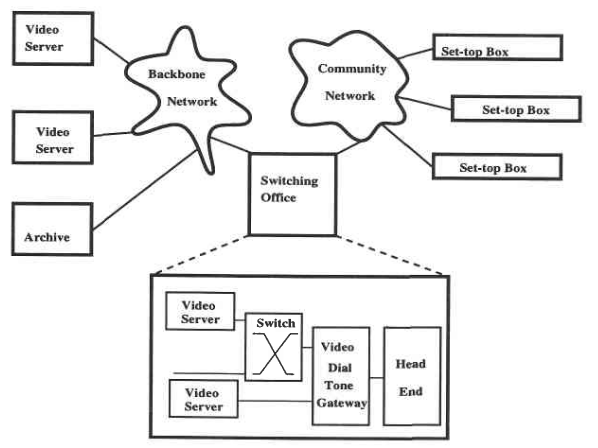
\includegraphics[width=0.8\textwidth]{vod}
	\caption{Video-On-Demand system.}\label{fig:vod}
\end{figure}
%--------------------------Figure end -------------------

\section{Video Conferencing}
Teleconferencing systems allow the user to achieve most of the efficiency and productivity of traditional meetings with one main difference: the user can stay at his/her desk as can the remote conference participants.

A multimedia conferencing system enables people to work together across geographically distant locations without the need to meet at one site. They communicate among each other in multi-party or face-to-face mode using motion video, audio and textual information in each direction. The audio and video quality heavily depends on the platform. Therefore, a big factor in the success of a teleconferencing system is to achieve high media quality over any platform and interconnectivity among various platforms and vendors. A possible setup of a video conferencing system is shown in Figure \ref{fig:video-conferencing}.

Video conferencing allows participants in a live session to see each other; the video is transmitted over the network between users, live and in real-time.

Video conferencing is used either in an office environment, where the video is displayed on a PC or workstation screen, or in a conference room, where the video is displayed on a \textit{video wall} (large TV screen).
%%%%%%%%%%%%%%%%%%%%%%%%%%%%%%%%%%%%%%%%%
%										%
%				FIGURE				   	%
%										%
%%%%%%%%%%%%%%%%%%%%%%%%%%%%%%%%%%%%%%%%%
\begin{figure}[hpt]
	\centering
	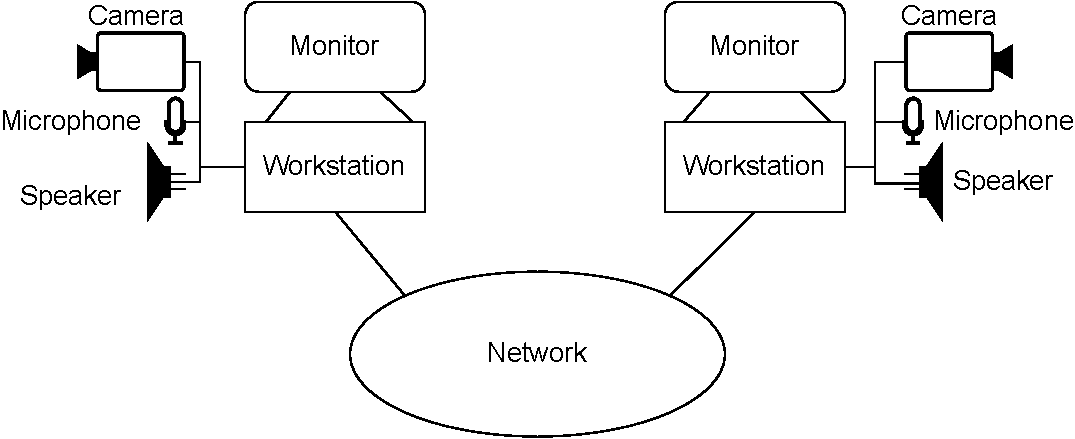
\includegraphics[width=0.8\textwidth]{video-conferencing}
	\caption{Video conferencing system.}\label{fig:video-conferencing}
\end{figure}
%--------------------------Figure end -------------------

Desktop video conferencing systems often include a dedicated shared white-board application. Application sharing denotes techniques which replicate the user interface of the
particular software (e.\ g.\ , the user's favorite text processor) so that the software can be used simultaneously by all participants of a conference. The concurrency in the
activities underlies the mechanisms of ``floor passing'' (also called ``chalk passing'') to determine which one of the users may actually interact with the software at a
given time.



\section{Educational Application, Industrial Application}
\subsection{Educational Application}
The world in which we live is changing rapidly and the field of education is experiencing these changes in particular as it applies to Media Services. The old days of an educational institution having an isolated audio-visual department are long gone! The growth in use of multimedia within the education sector has accelerated in recent years, and looks set for continued expansion in the future.


Teachers primarily require access to learning resources, which can support concept development by learners in a variety of ways to meet individual learning needs. The development of multimedia technologies for learning offers new ways in which learning can take place in schools and the home. Enabling teachers to have access to multimedia learning resources, which support constructive concept development, allows the teacher to focus more on being a facilitator of learning while working with individual students. Extending the use of multimedia learning resources to the home represents an educational opportunity with the potential to improve student learning.

The elements used in multimedia have all existed before. Multimedia simply combines these elements into a powerful new tool, especially in the hands of teachers and students. Interactive multimedia weaves five basic types of media into the learning environment: text, video, sound, graphics and animation. Since the mode of learning is interactive and not linear, a student or teacher can choose what to investigate next. For example, one does not start on the first page of a linear document and read to the end. Interactive multimedia learning mode is more like constructing a spider’s web, with one idea linked to another, allowing choices in the learner’s path.

The multimedia technologies that have had the greatest impact in education are those that augment the existing curriculum, allowing both immediate enhancement and encouraging further curriculum development. For example, the WWW serves as a storehouse of information that individual learners can search for subject matter content that specifically
fits their learning agendas. Multimedia applications for computers have been developed for single computing platforms such as the PC, Apple Mac and games machines.

\subsection{Industrial Application}
	\begin{itemize}
		\item Advertising
		\item Gaming industry
		\item Entertainment industry
		\item Fine arts
		\item Engineering
		\item Fashion design
		\item AI
	\end{itemize}



{\raggedright \section{Information System, Multimedia Archives \& Digital Libraries, Media Editors}\par}
 
 \subsection{Information Systems}
 Multimedia Information Systems (MIS) couple data management capabilities (effective and efficient methods for storage, indexing, querying, and retrieval) with media management (media representation, data compression, standardization, and transmission).
 
 Multimedia applications require representation and management of non-traditional data, such as text documents, images, audio and video data, possibly together with traditional (e.\ g.\ , relational or object-oriented) data. In particular, in multimedia applications, different data types are often coexisting within the same application domain. Hence, data management systems which are able to treat, in an integrated and uniform way, different types of data are needed.
 
 Multimedia information management systems, by definition, are not dealing with only a single media data type, but in fact need to be designed with the semantics and requirements of multiple media and modalities in mind. 
 
 A multimedia information system (MIS) architecture, consists of the following sub-systems: 
 
% \begin{multicols}{2}
 	 \begin{itemize}
 		\item a multimedia authoring system (MAS), 
 		\item a media sensing system (MSS),
 		\item media processing system (MPS),
 		\item multimedia communication system (MCS),
 		\item a multimedia visualization and interaction system 	
 		\item a multimedia object database (MODB)
 		\item a profile and context manager (PCM), and 
 		\item a digital rights management system (DRMS).
 	\end{itemize}
% \end{multicols}


\begin{enumerate}
	\item MAS is responsible for authoring of multimedia objects. This involves describing visual, temporal, spatial, hierarchical, and interactive properties of a
	complex multimedia object.
	
	\item  MSS uses environmentally distributed sensing	devices to collect multimedia data relevant for a given application.
	
	\item  MCS communicates media and multimedia objects between the various components of a multimedia
	information system, providing appropriate quality of service (QoS) guarantees.
	
	\item Since row, sensed data is often not directly usable,
	MPS processes media objects for the benefit of the
	other components. For example, multiple media
	objects may be fused to obtain a composite object,
	a media object may be processed to adjust its quality, or certain features may be extracted from a
	multimedia object for indexing purposes.
	
	\item  MVIS benefits from the user specifications to create	presentation schedules which maximize the utilization of available resources. It also enables the user
	to interact with the media objects and explore the	multimedia information space. It performs document and media scaling to match the resource requirements to the resource availabilities. It also benefits from document structure, priorities, user	preferences, and quality/cost trade-offs to develop object prefetching and caching strategies for document presentation.
	
	\item  MODB is responsible for storage and retrieval of	media objects and multimedia documents. MODB enables multimedia information to be queried and retrieved, efficiently and effectively. For this purpose it maintains appropriate index structures	to support queries. Since multimedia retrieval is subjective, unlike traditional databases, MODB employs fuzzy or probabilistic query processing techniques and ranking algorithms to present the query results according to their relevance
	
	\item PCM is responsible for keeping the user, context,	and task profiles to improve the processing and	presentation of multimedia information.
	
	
	\item DRSM ensures the intellectual property rights of	the users who contribute multimedia objects into the multimedia information system by providing	digital signatures and copy detection mechanisms.
\end{enumerate}


 \subsection{Multimedia Archives}
 The integration of multimedia archives through a common, unified access point for end users, always considering their particular copyright and access policies, emerges as a necessary step for the preservation of their content and their financial viability.
 
 During the last decade, the cost of storage and wide area communication services has decreased, while their capacity increased dramatically. This fact, along with the increasing penetration of e-commerce applications, has made digital storage, annotation and access of multimedia information a mature and viable choice for content holding organizations and individuals. Numerous multimedia archives have, either totally or incrementally, turned to the utilization of digitized archive technologies. The content of these archives can be made accessible, depending upon copyright, policy and security decisions, over the Internet in a cost-efficient, time efficient, anyplace, anytime fashion.
 
 However, one of the main problems of multimedia archiving has been inherited to their digital descendants. For traditional archives, where raw  media were stored in the form of analog hard copies, search was not an easy task as a human had to either go through a separate annotation archive, or, ideally, search using keywords in a custom, proprietary, metadata database. Much similarly to the case of books in a library that have not been indexed, information stored in a multimedia archive that cannot be searched, identified and accessed easily is practically unavailable.
 
 

\subsection{Digital Libraries}
 Digital Library is an information system targeted towards a specific community, where content from different sources is collected and managed, content is structured and enriched with metadata, and a set of services is offered that makes the content available to a user community via a communication network, typically the Internet.

 Digital Libraries are the electronic counterparts of traditional paper libraries, where the digital medium opens new opportunities, especially in the area of improved access support, increased content availability, powerful content interlinking, and reduced costs, but also imposes new challenges like long-term preservation in the context of fast changing storage technologies. Further important challenges are issues of copyright and digital rights management and the cost of digitization for not digitally-born content.
 
 
 A Digital Library is an information system targeted towards a specific community, where content from different sources is collected and managed, content is structured and enriched with metadata, and a set of services is offered that makes the content available to a user community via a communication network, typically the Internet. Multimedia Libraries are Digital Libraries, where the managed content is not restricted to the usually mainly textual documents. Such libraries contain, next to the ‘‘textual’’ contents, media types like music, videos, images, maps, and mixtures of different content types (multimedia objects) as they are, for example used in e-Learning or in the documentation of history. 
 
 Multimedia libraries may also contain content types that were not supported in traditional libraries at all like 3D objects, executable software (e.\ g.\ , computer games) or callable services. One of the main challenges for a multimedia library is to provide effective access to these types of context (based on adequate indexing) and to provide support for the ‘‘real-time’’ integration of different content types. Some challenges of multimedia libraries are closely related to those of museums and archives that make multimedia representations of their artifacts available online.
 
 

%A digital library, digital repository, or digital collection, is an online database of digital objects that can include text, still images, audio, video, digital documents, or other digital media formats. Objects can consist of digitized content like print or photographs, as well as originally produced digital content like word processor files or social media posts. In addition to storing content, digital libraries provide means for organizing, searching, and retrieving the content contained in the collection.

 
\subsection{Media Editors}
Media composition involves editing single media, i.\ e.\, changing its objects, such as characters, audio sentences, video frames and attributes such as the font of a
character, recording speed of an audio sentence or color of an image.

\begin{itemize}
	\item Text and Graphics editors
	\item Image editors
	\item Animation editors
	\item Sound editors
	\item Video editors
\end{itemize}

\subsubsection{Text Editors}
Text editors provide writing and modifying facilities to compose text in a document. There are either separate text editors (e.\ g.\ , Emacs, Vim, Nano text editor in combination  with the \LaTeX\footnote{\textnp{याे पूरै नाेट तयार पार्न पनि {\LaTeX} नै प्रयाेग गरिएकाे छ।} \url{https://www.latex-project.org/}} document preparation tool on workstations, LibreWriter on PCs) or text is embedded in graphical tools such as drawing programs CorelDRAW.


An example of an advanced word processor with graphical capabilities is \textit{Microsoft Word}, \textit{Libre Writer}. These tools provides, in addition to text capabilities, a new toolbar and ribbon that can be customized for the creation oftables, envelopes, bullets and more.

\subsubsection{Graphics Editors}
Graphics editors use facilities at the user interface for editing structural representations of graphical objects (structure-level editing) and for modifying higher-level
operations on graphical objects (object-level editing). These two levels of editing are possible because the graphical system stores object primitives and their structural
representations, which can be manipulated. These drawing application, are also called \textit{layout editor} or \textit{graphical illustrator}. Example Adobe Illustrator, CorelDRAW, etc.


\subsubsection{Image Editors}
Image editors are suitable for applications when neither the application nor the underlying software package keeps a record of the primitives (as is typical in most
painting programs).

An example of a graphics/image editor is \textit{Adobe Photoshop}. This tool allows one to draw, edit and paste objects on several layers. Experimenting with different
combinations of graphics, text and special effects without altering the original background image is possible. Furthermore, Filters let the user create 3D lighting
effects, and remove dust and scratches from scanned images.

\subsubsection{Animation Editors}
Animation editing is based on graphical editors with respect to 2D or 3D spatial graphic objects. The additional component in animation is time, which can also be edited (4D editing). The functionalities of such editors include c\textit{utting frames from an animation clip}, \textit{adding new frames to an animation clip}, etc.

The animation tools provide the animator with the capability to draw only the key frame. The intermediate frames are then drawn by the computer animation program. This process is called \textit{tweening}. Further, some animation tools include morphing (polymorphic tweening), which is a transformation from one shape to another. With this technique, many special effects can be created.


\subsubsection{Sound Editors}
Sound tools support a number of operations that let the user access, modify and play sound data. The operations fall into following categories:
\begin{enumerate}
	\item \textit{Locating and Storing Sounds}
	\item \textit{Recording and Playback}
	\item \textit{Editing}
\end{enumerate}

\paragraph*{Locating and Storing Sounds}
Location and storage of sounds can be done in four ways: 
\begin{enumerate}
	\item \textit{record} a sound using an A/D audio device (analog-to-digital converter), 
	\item \textit{read} sound data from a sound file,
	\item \textit{retrieve} a sound from a pasteboard, and 
	\item \textit{create} sound data algorithmically.
\end{enumerate}

\paragraph*{Recording and Playback}
The record operation continuously records sound from a microphone input until it is stopped or paused. Recorded sound is \textit{m-law encoded}. The data are sampled at a rate of 8000 samples per second with 12-bit precision, but if the digitized sound is being compressed, then 8-bit precision per sample is achieved.

The playback operation plays a sound using a D/A audio device (digital-to-analog converter) speaker output.

\paragraph*{Editing}
The editing operation allows one to copy/paste, cut, delete, insert or replace sampled sound data. One problem ought to be pointed out here: audio data are normally contiguous in memory. However, when a sound object is edited, its data can become fragmented or discontiguous. Fragmented sounds are played less efficiently. Hence, it is important to have an operation which compacts the samples into a contiguous object.


\subsubsection{Video Editors}
Video editors are based on image editors for editing individual frames, but as in the case of animation editing, temporal considerations are important. Therefore, time resolution (time aliasing) is solved if frames are deleted, added or replaced. Editing functionalities of video editors may combine several cuts into one sequence, adjust
audio separately from video and add video transition effects. An example of such a motion video editor is \textit{Adobe Premiere}, \textit{Edius}, \textit{Final Cut}, \textit{Kdenlive} etc.

In the case of a conventional videotape, the edited sequence of video frames must be recorded to a new tape to view the new video clip. This kind of editing is called \textit{linear editing}. Video editor provides an \textit{Edit Decision List (EDL)} from which the final video can be reconstructed, i.\ e.\ , the edited video does not have to be recorded to a new tape because it can be played continuously using the EDL. This is called \textit{non-linear editing}. Such tools have further editing capabilities, e.\ g.\, adding dynamic transitions such as wipes, dissolves or fades between cuts.

Video editors include several editors for editing video, sound and music in an integrated fashion.

\newpage\thispagestyle{empty}